\documentclass[aspectratio=169]{beamer}

\usetheme{Boadilla}
\usefonttheme{professionalfonts}
\setbeamertemplate{navigation symbols}{}
\setbeamertemplate{itemize items}[circle]
\setbeamertemplate{enumerate items}[default]
\setbeamertemplate{headline}{}

\usepackage[utf8]{inputenc}
\usepackage[T1]{fontenc}
\usepackage{lmodern}
\usepackage{amsmath}
\usepackage{booktabs}
\usepackage{tabularx}
\usepackage{array}
\usepackage{hyperref}
\usepackage[strings]{underscore}
\usepackage{listings}
\usepackage{tikz}
\usetikzlibrary{arrows.meta,positioning,fit,calc,shapes.geometric}
\usepackage{xcolor}

\definecolor{courseblue}{HTML}{12355B}
\definecolor{coursegold}{HTML}{C98A2E}
\definecolor{courseice}{HTML}{EEF3F8}
\definecolor{coursegreen}{HTML}{2F6B4F}
\definecolor{coursegray}{HTML}{4B5563}
\definecolor{codebg}{HTML}{F7F9FC}
\definecolor{codecomment}{HTML}{5E6C84}
\definecolor{codestring}{HTML}{0B6E4F}

\setbeamercolor{palette primary}{bg=courseblue,fg=white}
\setbeamercolor{palette secondary}{bg=coursegold,fg=white}
\setbeamercolor{palette tertiary}{bg=courseblue,fg=white}
\setbeamercolor{palette quaternary}{bg=coursegold,fg=white}
\setbeamercolor{structure}{fg=courseblue}
\setbeamercolor{frametitle}{bg=courseice,fg=courseblue}
\setbeamercolor{title}{fg=courseblue}
\setbeamercolor{block title}{bg=courseblue,fg=white}
\setbeamercolor{block body}{bg=courseice,fg=black}
\setbeamercolor{normal text}{fg=black,bg=white}
\setbeamercolor{alerted text}{fg=coursegold}

\setbeamerfont{footline}{size=\scriptsize}

\setbeamertemplate{footline}{
  \leavevmode
  \hbox{
    \begin{beamercolorbox}[wd=.33\paperwidth,ht=2.8ex,dp=1.2ex,leftskip=0.8em]{palette primary}%
      University of Trieste
    \end{beamercolorbox}%
    \begin{beamercolorbox}[wd=.49\paperwidth,ht=2.8ex,dp=1.2ex,center]{palette tertiary}%
      \coursename{} \textbar{} \coursecode
    \end{beamercolorbox}%
    \begin{beamercolorbox}[wd=.18\paperwidth,ht=2.8ex,dp=1.2ex,rightskip=0.8em plus1fil]{palette secondary}%
      \insertframenumber{} / \inserttotalframenumber
    \end{beamercolorbox}%
  }
}

\hypersetup{
  colorlinks=true,
  linkcolor=courseblue,
  urlcolor=coursegreen
}

\lstdefinestyle{coursepython}{
  language=Python,
  basicstyle=\ttfamily\footnotesize,
  keywordstyle=\color{courseblue}\bfseries,
  commentstyle=\color{codecomment}\itshape,
  stringstyle=\color{codestring},
  showstringspaces=false,
  columns=fullflexible,
  keepspaces=true,
  frame=single,
  framerule=0.6pt,
  rulecolor=\color{courseblue},
  backgroundcolor=\color{codebg},
  xleftmargin=0.4em,
  xrightmargin=0.4em,
  aboveskip=0.4em,
  belowskip=0.2em
}

\newcommand{\coursename}{Data-driven Systems Engineering}
\newcommand{\coursecode}{440MI / 305SM}
\newcommand{\coursefooter}{}

\newcommand{\learninggoals}[1]{
  \begin{block}{Learning goals}
  #1
  \end{block}
}

\newcommand{\repoactivity}[1]{
  \begin{block}{Repo activity}
  #1
  \end{block}
}

\newcommand{\readinglist}[1]{
  \begin{block}{Papers and materials}
  {\footnotesize #1}
  \end{block}
}

\newcommand{\coursecontextframe}[5]{
  \begin{frame}{Course Map and Running Cases}
  \centering
  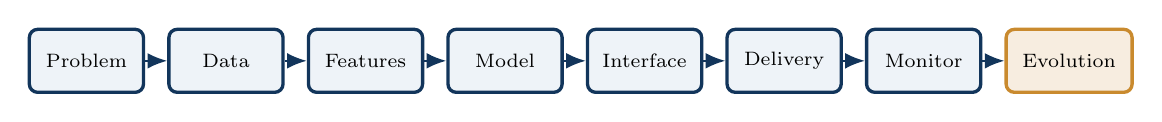
\begin{tikzpicture}[node distance=0.28cm]
  \node[flowbox, minimum width=1.45cm, minimum height=0.8cm] (problem) {\scriptsize Problem};
  \node[flowbox, minimum width=1.45cm, minimum height=0.8cm, right=of problem] (data) {\scriptsize Data};
  \node[flowbox, minimum width=1.45cm, minimum height=0.8cm, right=of data] (features) {\scriptsize Features};
  \node[flowbox, minimum width=1.45cm, minimum height=0.8cm, right=of features] (model) {\scriptsize Model};
  \node[flowbox, minimum width=1.45cm, minimum height=0.8cm, right=of model] (interface) {\scriptsize Interface};
  \node[flowbox, minimum width=1.45cm, minimum height=0.8cm, right=of interface] (delivery) {\scriptsize Delivery};
  \node[flowbox, minimum width=1.45cm, minimum height=0.8cm, right=of delivery] (monitor) {\scriptsize Monitor};
  \node[accentbox, minimum width=1.6cm, minimum height=0.8cm, right=of monitor] (evolution) {\scriptsize Evolution};
  \foreach \a/\b in {problem/data,data/features,features/model,model/interface,interface/delivery,delivery/monitor,monitor/evolution} {
    \draw[arrow] (\a) -- (\b);
  }
  \end{tikzpicture}

  \vspace{0.5em}
  \begin{block}{Today in the course}
  \textbf{Focus:} #1

  \textbf{Bridge:} #2
  \end{block}

  \begin{columns}[T]
  \column{0.48\textwidth}
  \begin{block}{Fraud case}
  {\footnotesize #3}
  \end{block}
  \column{0.48\textwidth}
  \begin{block}{Pasteurization case}
  {\footnotesize #4}
  \end{block}
  \end{columns}

  \vspace{0.3em}
  {\footnotesize \textbf{Course thread:} #5}
  \coursefooter
  \end{frame}
}

\newcommand{\classclosingframe}[4]{
  \begin{frame}{From This Class to the Next}
  \begin{block}{What stays with us}
  #1
  \end{block}

  \begin{columns}[T]
  \column{0.48\textwidth}
  \begin{block}{Project use}
  {\footnotesize #2}
  \end{block}
  \column{0.48\textwidth}
  \begin{block}{Next connection}
  {\footnotesize #3}
  \end{block}
  \end{columns}

  \vspace{0.3em}
  {\footnotesize \textbf{Course thread:} #4}
  \coursefooter
  \end{frame}
}

\tikzset{
  flowbox/.style={
    rounded corners=3pt,
    draw=courseblue,
    fill=courseice,
    very thick,
    minimum width=2.2cm,
    minimum height=0.9cm,
    align=center,
    font=\small
  },
  accentbox/.style={
    rounded corners=3pt,
    draw=coursegold,
    fill=coursegold!15,
    very thick,
    minimum width=2.2cm,
    minimum height=0.9cm,
    align=center,
    font=\small
  },
  arrow/.style={
    -{Latex[length=2.5mm,width=2mm]},
    thick,
    draw=courseblue
  }
}


\title{Class 15: Feature Engineering: Cleaning, Curation, Selection, Construction}
\author{\coursename}
\date{}

\begin{document}

\frame{\titlepage \coursefooter}

\begin{frame}{Agenda}
\begin{itemize}
\item Why feature engineering is still necessary once data is already encoded.
\item Data cleaning: missingness, duplicates, and typed filling.
\item Data curation: documenting and validating datasets for reuse.
\item Feature selection: filter, wrapper, and embedded methods.
\item Feature construction from domain knowledge, for tables and for streams.
\item Leakage and availability checks before anything ships.
\end{itemize}
\coursefooter
\end{frame}

\begin{frame}{Learning goals}
\learninggoals{
\begin{itemize}
\item Distinguish cleaning, curation, selection, and construction as separate engineering tasks.
\item Apply filter, wrapper, and embedded feature selection appropriately.
\item Construct new features from domain logic rather than generic transformations.
\item Recognize leakage and feature-availability problems before they reach production.
\end{itemize}
}
\coursefooter
\end{frame}

\coursecontextframe
{Cleaning, curating, selecting, and constructing features once variables are already numeric.}
{Class 14 gave us a numeric representation of every variable. This class decides which of those variables to keep, fix, or build into something more useful.}
{In the fraud case, feature work means fixing data-quality issues, keeping only informative variables, and building indicators such as spending deviation from a rolling baseline.}
{In the pasteurization case, feature work means validating sensor readings and constructing rate-of-change and state-aware variables such as `dTdt`.}
{After this class, the course can talk about model quality because the input representation has already been made explicit and deliberate.}

\begin{frame}{Why feature engineering still matters after encoding}
\begin{itemize}
\item Encoding (Class 14) only makes a variable numeric; it says nothing about whether that variable is clean, trustworthy, or worth keeping.
\item Many real datasets carry missing values, duplicates, and inconsistent types that must be resolved before any encoding decision is meaningful.
\item Not every available column deserves to be a feature: some are redundant, some are noise, and some are actively misleading.
\item The best features are often not present in the raw data at all; they must be constructed from domain knowledge.
\end{itemize}
\coursefooter
\end{frame}

\begin{frame}{Four related but different tasks}
\begin{tabularx}{\textwidth}{>{\bfseries}l X}
Cleaning & Fix missingness, duplicates, invalid values, and basic type errors. \\
Curation & Organize, document, and validate datasets so they can be reused and trusted. \\
Selection & Keep the most informative existing variables and drop the rest. \\
Construction & Build new features from domain logic, time, aggregation, or combinations. \\
\end{tabularx}
\coursefooter
\end{frame}

\begin{frame}{Data cleaning}
\begin{itemize}
\item Start by inventorying missingness, duplicates, and data types before making any modeling decision.
\item Missing-value policy should depend on column meaning, not a single global rule.
\item Some categorical columns are better served by an explicit ``Unknown'' category than by imputation.
\item Cleaning decisions must be documented, because they change the meaning of the data for everyone downstream.
\end{itemize}
\coursefooter
\end{frame}

\begin{frame}[fragile]{Cleaning example: typed, column-aware filling}
\begin{lstlisting}[style=coursepython]
titanic = titanic.dropna(subset=["survived"])

for col in ["deck", "embark_town"]:
    titanic[col] = titanic[col].astype("category")
    titanic[col] = titanic[col].cat.add_categories("Unknown")
    titanic[col] = titanic[col].fillna("Unknown")

titanic["age"] = titanic["age"].fillna(titanic["age"].median())
titanic["embarked"] = titanic["embarked"].fillna("S")
\end{lstlisting}
\begin{itemize}
\item From `notebooks/Class4_DataEngineering.ipynb`: three different missingness policies for three different column types in the same dataset.
\item Dropping rows, adding an explicit category, and median imputation are all defensible, but only for the right column.
\end{itemize}
\coursefooter
\end{frame}

\begin{frame}{Data curation}
\begin{itemize}
\item Curation is what makes a cleaned dataset reusable by someone other than the person who cleaned it.
\item A data dictionary records what every column means, its unit, and its valid range.
\item Versioning the dataset (or at least recording an extraction date) lets later experiments be compared fairly.
\item Validation rules (schema checks, range checks) catch upstream problems before they reach modeling.
\end{itemize}
\begin{block}{Repository example}
The fraud case's supporting specification in `documents/` plays the role of a curated data description: it documents the dataset and workflow rather than leaving them implicit in a notebook.
\end{block}
\coursefooter
\end{frame}

\begin{frame}{Feature selection: filter, wrapper, embedded}
\begin{tabularx}{\textwidth}{>{\bfseries}l X}
Filter & Score each feature independently of any model (correlation, chi-squared) and drop low scorers. \\
Wrapper & Search over feature subsets by repeatedly training and evaluating a model. \\
Embedded & Let the model itself assign importance during training (Lasso coefficients, tree feature importances). \\
\end{tabularx}
\coursefooter
\end{frame}

\begin{frame}[fragile]{Filter example: chi-squared scores for categorical features}
\begin{lstlisting}[style=coursepython]
encoded = pd.DataFrame()
for col in cat_features.columns:
    le = LabelEncoder()
    encoded[col] = le.fit_transform(cat_features[col].astype(str))

chi_scores, p_values = chi2(encoded, y)
\end{lstlisting}
\begin{itemize}
\item From `notebooks/Class4_DataEngineering.ipynb`: chi-squared is a filter method, computed once, before any model is trained.
\item It ranks categorical features by their statistical association with the target, independent of model choice.
\end{itemize}
\coursefooter
\end{frame}

\begin{frame}{Notebook plot: chi-squared scores for categorical features}
\centering
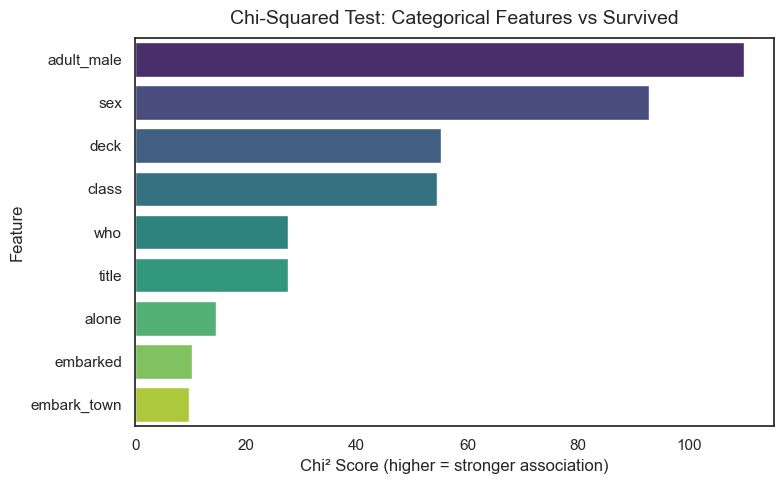
\includegraphics[height=0.72\textheight]{images/class04_chi2_feature_scores.png}

{\scriptsize From `Class4_DataEngineering.ipynb`: not every available categorical feature contributes equally to predicting the outcome.}
\coursefooter
\end{frame}

\begin{frame}[fragile]{Selection example: dropping a redundant feature}
\begin{lstlisting}[style=coursepython]
# Remove correlated or redundant features
# Example: drop 'is_alone' if family_size already encodes similar info
print(X.shape)
X_selected = X.drop(columns=["is_alone"])
print(X_selected.shape)
\end{lstlisting}
\begin{itemize}
\item This is a manual, knowledge-driven form of selection: `is_alone` is largely redundant once `family_size` is present.
\item Selection does not always need an automated score; sometimes domain reasoning is the fastest filter.
\end{itemize}
\coursefooter
\end{frame}

\begin{frame}{Feature construction from domain knowledge}
\begin{itemize}
\item The best new features usually come from understanding the problem, not from generic mathematical transforms.
\item Aggregation (counts, sums), ratios, and simple domain rules often outperform complex automated feature generation.
\item Constructed features should be checked for redundancy against the columns that produced them.
\item Students should be able to explain, in one sentence, why a constructed feature should help the model.
\end{itemize}
\coursefooter
\end{frame}

\begin{frame}[fragile]{Construction example: simple domain logic}
\begin{lstlisting}[style=coursepython]
titanic["family_size"] = titanic["sibsp"] + titanic["parch"] + 1
titanic["is_alone"] = (titanic["family_size"] == 1).astype(int)
titanic["title"] = titanic["who"].map(
    {"man": "Mr", "woman": "Mrs", "child": "Master"}
)
\end{lstlisting}
\begin{itemize}
\item From `notebooks/Class4_DataEngineering.ipynb`: each new column is a short, explainable rule, not a black-box transformation.
\item Richer examples for the fraud case: rolling transaction count, deviation from recent spending, merchant risk history.
\end{itemize}
\coursefooter
\end{frame}

\begin{frame}{Feature construction for streams and sensors}
\begin{itemize}
\item Instantaneous sensor values are often less informative than trends and rates of change.
\item Window-based features such as rolling means can reveal process stability that a single reading cannot.
\item State-aware features distinguish normal variation within a phase from a genuine anomaly.
\item Streaming systems must compute these features online, one observation at a time, not only offline in a notebook.
\end{itemize}
\begin{block}{Repository example}
`pasteurization/synth_sensors.py` already includes the derived feature `dTdt`, a simple but meaningful process feature built from raw temperature.
\end{block}
\coursefooter
\end{frame}

\begin{frame}{Notebook plot: engineered features change the picture}
\centering
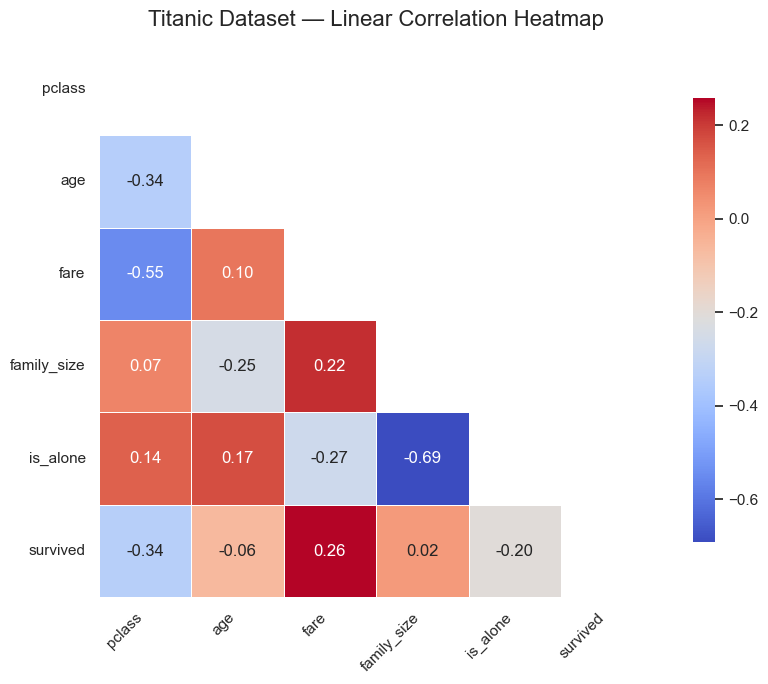
\includegraphics[height=0.72\textheight]{images/class04_engineered_feature_heatmap.png}

{\scriptsize From `Class4_DataEngineering.ipynb`: constructed variables such as `family_size` and `title` change how features relate to the target compared to the raw columns alone.}
\coursefooter
\end{frame}

\begin{frame}{Leakage and availability checks}
\begin{itemize}
\item Was this feature actually available at prediction time, or does it use information from the future?
\item Does it encode a post-decision outcome, such as a manual review result?
\item Will the feature be computed the same way in production as it was in the notebook?
\item Does the feature depend on unstable joins or upstream systems that may not always be available?
\end{itemize}
\coursefooter
\end{frame}

\begin{frame}{Repository connections}
\repoactivity{
\begin{itemize}
\item `notebooks/Class4_DataEngineering.ipynb` covers cleaning, chi-squared selection, and domain-driven construction end to end.
\item `pasteurization/synth_sensors.py` is the constructed-feature example for time series data (`dTdt`).
\item `streamlit/modeling.py` shows why cleaning and construction decisions must be saved alongside the model, not just applied once in a notebook.
\end{itemize}
}
\coursefooter
\end{frame}

\begin{frame}{Discussion prompt}
\begin{block}{Question}
`is_alone` was dropped as redundant with `family_size`. Is that selection decision purely statistical, or does it also depend on domain reasoning?
\end{block}
\begin{itemize}
\item This distinguishes filter-style automated selection from the domain judgment that guided construction in the first place.
\end{itemize}
\coursefooter
\end{frame}

\begin{frame}{Papers and materials}
\readinglist{
\href{https://www.oreilly.com/library/view/feature-engineering-for/9781491953235/}{Zheng and Casari, Feature Engineering for Machine Learning};\
\href{https://dl.acm.org/doi/10.1145/2347736.2347755}{Domingos (2012), A Few Useful Things to Know About Machine Learning};\
\href{https://scikit-learn.org/stable/modules/compose.html}{scikit-learn pipelines and composite estimators};\
\href{https://pandas.pydata.org/docs/}{pandas documentation}.
}
\coursefooter
\end{frame}

\classclosingframe
{\begin{itemize}
\item Cleaning, curation, selection, and construction are four distinct tasks, each with its own failure modes.
\item Filter, wrapper, and embedded selection methods answer ``which features to keep'' in different, complementary ways.
\item The strongest features usually come from domain knowledge, not automated transformation alone.
\end{itemize}}
{Project teams should now be able to justify which raw variables were cleaned, kept, dropped, or constructed, and defend each choice on evidence or domain logic.}
{Class 16 turns this feature set into model comparisons, and pairs modeling with disciplined experiment tracking and tuning.}
{Well-engineered features turn modeling from guesswork into a principled comparison between alternatives.}

\end{document}
